% Autor: Leonhard Segger, Alexander Neuwirth
% Datum: 2017-10-30
\documentclass[
	% Papierformat
	a4paper,
	% Schriftgröße (beliebige Größen mit „fontsize=Xpt“)
	12pt,
	% Schreibt die Papiergröße korrekt ins Ausgabedokument
	pagesize,
	% Sprache für z.B. Babel
	ngerman
]{scrartcl}

% Achtung: Die Reihenfolge der Pakete kann (leider) wichtig sein!
% Insbesondere sollten (so wie hier) babel, fontenc und inputenc (in dieser
% Reihenfolge) als Erstes und hyperref und cleveref (Reihenfolge auch hier
% beachten) als Letztes geladen werden!

% Silbentrennung etc.; Sprache wird durch Option bei \documentclass festgelegt
\usepackage{babel}
% Verwendung der Zeichentabelle T1 (Sonderzeichen etc.)
\usepackage[T1]{fontenc}
% Legt die Zeichenkodierung der Eingabedatei fest, z.B. UTF-8
\usepackage[utf8]{inputenc}
% Schriftart
\usepackage{lmodern}
% Zusätzliche Sonderzeichen
\usepackage{textcomp}

% Mathepaket (intlimits: Grenzen über/unter Integralzeichen)
\usepackage[intlimits]{amsmath}
% Ermöglicht die Nutzung von \SI{Zahl}{Einheit} u.a.
\usepackage{siunitx}
% Zum flexiblen Einbinden von Grafiken (\includegraphics)
\usepackage{graphicx}
% Abbildungen im Fließtext
\usepackage{wrapfig}
% Abbildungen nebeneinander (subfigure, subtable)
\usepackage{subcaption}
% Funktionen für Anführungszeichen
\usepackage{csquotes}
% Zitieren, Bibliographie
\usepackage{biblatex}


% Zur Darstellung von Webadressen
\usepackage{url}
%chemische Formeln
\usepackage[version=4]{mhchem}
% siunitx: Deutsche Ausgabe, Messfehler getrennt mit ± ausgeben
\usepackage{floatrow}
\floatsetup[table]{capposition=top}
\usepackage{float}
% Verlinkt Textstellen im PDF-Dokument
\usepackage[unicode]{hyperref}
% "Schlaue" Referenzen (nach hyperref laden!)
\usepackage{cleveref}
\sisetup{
	locale=DE,
	separate-uncertainty
}
\bibliography{14Mo_O7_23-04-2018_References}

\begin{document}
	
	\begin{titlepage}
		\centering
		{\scshape\LARGE Versuchsbericht zu \par}
		\vspace{1cm}
		{\scshape\huge O7 - Beugung am Spalt, Doppelspalt und Gitter \par} %TODO Anpasen
		\vspace{2.5cm}
		{\LARGE Gruppe 14Mo \par}
		\vspace{0.5cm}
		
		{\large Alexander Neuwirth (E-Mail: a\_neuw01@wwu.de) \par}
		{\large Leonhard Segger (E-Mail: l\_segg03@uni-muenster.de) \par}
		\vfill
		
		durchgeführt am 23.04.2018\par %TODO Anpassen
		betreut von\par
		{\large Lukas Britt} %TODO Anpassen
		
		\vfill
		
		{\large \today\par}
	\end{titlepage}
	\tableofcontents
	\newpage

	\section{Kurzfassung}
	%TODO Hypothese	und deren Ergebnis
	%TODO Ergebnisse, auch Zahlen, mindestens wenn's halbwegs Sinn ergibt
	%TODO Was wurde gemacht
	
	\section{Methoden}
	%TODO Bilder von der Website klauen
	In \cref{optischeBank} ist er Aufbau des Experiments illustriert.
	An einem Ende der optischen Bank befindet sich ein Diodenlaser und davor ein Polarisator und der Halter für Spalte.
	Am anderen Ende der optischen Bank ist eine durch eine Kurbel senkrecht zu optischen Bank zu bewegende Photodiode angebracht.
	Die Halterung der Photodiode ist über ein Seil mit einem Rad verbunden, um die Intensitätsmessung der Diode mit der Position der Diode im Strahlengang zu verbinden.
	Nun kann eine Spaltanordnung in die Halterung gebracht werden und durch Bewegung der Photodiode über die optische Bank die Intensitätsverteilung der Spalte bestimmt werden.
	Dies wurde für unterschiedliche Spalte durchgeführt. %TODO Neukalibrierung erwähnen?
	
	\begin{figure}[H]
		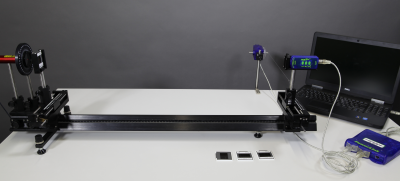
\includegraphics[width=0.7\textwidth]{optischeBank}
		\centering
		\caption{Aufbau der optischen Bank. Auf der linken Seite sind Laser und Beugungsanordnung und auf der rechten Seite die Photodiode zu sehen.\cite{optischeBank} }
		\label{optischeBank}
		\centering
	\end{figure} 
	
	\section{Ergebnisse und Diskussion}
	%TODO Datenanalyse -> Überschrift?
	%TODO Unsicherheiten
	

	\subsection{Beobachtung}

	\subsection{Diskussion}
	%TODO Bezug/Nutzten oder sonst was
	%TODO auch hier die Hypothese wiederholen
	
	\section{Schlussfolgerung}
	%TODO Rückgriff auf Hypothese und drittes Nennen dieser
	
	%TODO Quellen zitieren, Websiten mit Zugriffsdatum
	%TODO Verweise auf das Laborbuch (sind erlaubt)
	%TODO Tabelle + Bilder mit Beschriftung
	\printbibliography
\end{document}
